\documentclass[conference]{IEEEtran}
% BẮT BUỘC XeLaTeX. Overleaf: Menu → Settings → Compiler → XeLaTeX

\usepackage{array}
\usepackage{fontspec}
\setmainfont{Times New Roman}
\setmonofont{Courier New}

\usepackage[vietnamese]{babel}
\usepackage{amsmath,amssymb,amsfonts}
\usepackage{graphicx}
\usepackage{xcolor}
\usepackage{booktabs}
\usepackage{multirow}
\usepackage{subcaption}
\usepackage{caption}
\captionsetup[figure]{
  font=small,
  labelfont=normalfont,
  textfont=normalfont,
  justification=centering,
  singlelinecheck=false,
  labelsep=period
}
\usepackage{hyperref}
\usepackage{listings}
\usepackage{adjustbox}

\graphicspath{{images/}}

\lstset{
  basicstyle=\ttfamily\footnotesize,
  breaklines=true,
  frame=single,
  backgroundcolor=\color{gray!10},
  captionpos=b
}

\begin{document}

\title{MedCLIP-SAMv2: Hướng tới phân đoạn ảnh y khoa phổ quát điều khiển bằng văn bản}

\author{
    \IEEEauthorblockN{%
        \centering\small
        \begin{tabular*}{\linewidth}{@{\extracolsep{\fill}}cccc@{}}
            \begin{tabular}[t]{c}
                \textbf{1. Thiều Đinh Nam Tài} \\
                \textit{MSSV: 23521378}
            \end{tabular} &
            \begin{tabular}[t]{c}
                \textbf{2. Huỳnh Trần Anh Thư} \\
                \textit{MSSV: 23521535}
            \end{tabular} &
            \begin{tabular}[t]{c}
                \textbf{3. Nguyễn Lan Hương} \\
                \textit{MSSV: 23520588}
            \end{tabular} &
            \begin{tabular}[t]{c}
                \textbf{4. Nguyễn Trung Duy} \\
                \textit{MSSV: 22520335}
            \end{tabular}
        \end{tabular*}
    }

    \vspace{0.5cm}

    \IEEEauthorblockN{\textbf{Giảng viên hướng dẫn:} ThS. Dương Phi Long; KS. Phạm Nguyễn Thanh Bình}

    \vspace{0.2cm}
    \IEEEauthorblockA{
        \textit{Trường Đại học Công nghệ Thông tin}\\
        Đại học Quốc gia TP.HCM, Việt Nam
    }
}

\maketitle
\thispagestyle{plain}
\pagestyle{plain}

\begin{abstract}
Báo cáo trình bày việc tái hiện framework \textbf{MedCLIP-SAMv2} (Koleilat \textit{et al.}, arXiv:2409.19483)---phân đoạn ảnh y khoa đa phương thức chỉ bằng mô tả văn bản lâm sàng, kết hợp fine-tune BiomedCLIP (DHN-NCE), saliency M2IB, Segment Anything Model (SAM) và huấn luyện yếu giám sát nnUNet với ensemble checkpoint. Nhóm triển khai pipeline ba giai đoạn trên Windows, GPU RTX 4060 Ti 16\,GB, bốn bộ dữ liệu (siêu âm vú, MRI não, X-quang và CT phổi), so sánh DSC/NSD với bài báo gốc. Kết quả tái hiện cho thấy X-quang đạt DSC zero-shot khoảng 50\% (bài báo $\sim$76\%), các modality còn lại $\sim$5--9\%; phân tích nguyên nhân và trực quan hóa được trình bày theo cấu trúc: bài toán, phương pháp, thực nghiệm (gốc / tái hiện / mở rộng).
\end{abstract}

\begin{IEEEkeywords}
Medical Image Segmentation, MedCLIP-SAMv2, BiomedCLIP, SAM, M2IB, nnUNet, Zero-Shot, Weakly Supervised Learning.
\end{IEEEkeywords}

%==============================================================================
\section{Giới thiệu}
\label{sec:gioithieu}
%==============================================================================

Phân đoạn ảnh y tế (Medical Image Segmentation) đóng vai trò cốt lõi trong quy trình hỗ trợ chẩn đoán lâm sàng, lập kế hoạch điều trị và theo dõi tiến triển bệnh lý. Mặc dù các mô hình học sâu truyền thống dựa trên kiến trúc Fully Convolutional Networks (FCN) hoặc U-Net đã đạt được những thành tựu vượt bậc, chúng vẫn bộc lộ những hạn chế nghiêm trọng về tính linh hoạt: mô hình thường bị bó hẹp trong một loại cơ quan hoặc một phương thức hình ảnh y tế cố định và đòi hỏi lượng dữ liệu gán nhãn pixel-level vô cùng lớn.

Nhằm giải quyết triệt để rào cản này, framework MedCLIP-SAMv2~\cite{ref1} được đề xuất như một giải pháp, tích hợp khả năng hiểu ngữ nghĩa đa phương thức của mô hình nền tảng y sinh BioMedCLIP~\cite{ref3} và Segment Anything Model (SAM)~\cite{ref2,ref4}. Sự kết hợp này mở ra phương pháp phân đoạn ảnh y tế dựa trên gợi ý văn bản (text-driven segmentation), cho phép người dùng điều khiển mô hình thông qua các câu lệnh (prompt) bằng ngôn ngữ tự nhiên mô tả thực thể bệnh học.

Mô hình thể hiện ưu thế ở cả hai kịch bản phân đoạn không cần huấn luyện (zero-shot segmentation) và phân đoạn giám sát yếu (weakly supervised segmentation)~\cite{ref1} trên đa dạng các phương thức chẩn đoán hình ảnh (modalities) như Siêu âm (Ultrasound), Cộng hưởng từ (MRI), Cắt lớp vi tính (CT), và X-quang (X-ray). Báo cáo này tập trung phân tích kiến trúc hệ thống, các cải tiến cốt lõi từ bài báo gốc, đồng thời ghi nhận kết quả từ kho lưu trữ thực nghiệm cá nhân được triển khai trên môi trường phần cứng cục bộ.

\vspace{0.4em}
\begin{center}
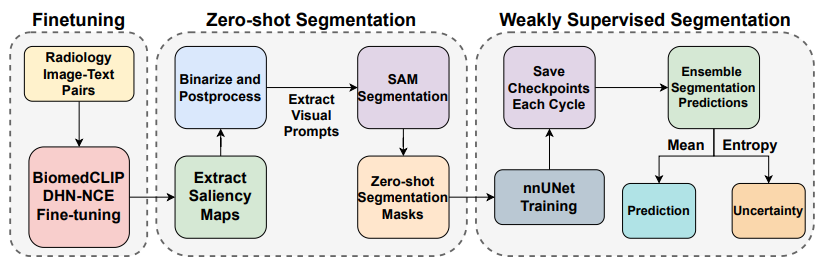
\includegraphics[width=\linewidth,keepaspectratio]{KienTrucTQuanMedClip.png}
\captionof{figure}{\normalfont Mô hình hóa ý tưởng text-driven medical image segmentation kết hợp giữa Vision-Language Models (BioMedCLIP) và Foundation Models cho phân đoạn ảnh (SAM)~\cite{ref1}.}
\label{fig:kientruc}
\end{center}
\vspace{0.3em}

%==============================================================================
\section{Mục tiêu nghiên cứu}
\label{sec:muctieu}
%==============================================================================

Phân tích và tái hiện pipeline MedCLIP-SAMv2~\cite{ref1} từ bài báo gốc, không đề xuất kiến trúc mới. Các mục tiêu chính bao gồm:

\begin{itemize}
    \item Nghiên cứu sâu kiến trúc hệ thống: Phân tích cơ chế liên kết đa phương thức giữa mô hình mã hóa ngôn ngữ-hình ảnh y tế (BioMedCLIP)~\cite{ref3} và mô hình phân đoạn hình học (SAM)~\cite{ref2,ref4}, đặc biệt là vai trò trung gian của khối nghẽn thông tin đa phương thức (Multi-modal Information Bottleneck - M2IB)~\cite{ref7}.
    \item Tái hiện thành công thực nghiệm: Triển khai mã nguồn từ bài báo gốc, cấu hình môi trường phần cứng cục bộ và tối ưu hóa quy trình chạy pipeline zero-shot từ kho lưu trữ Blackdarked/MedCLIP-SAMv2~\cite{ref1}.
    \item Đánh giá hiệu quả định lượng: Đo lường năng lực phân đoạn dựa trên các chỉ số tiêu chuẩn của ngành y tế (Dice Coefficient, Intersection over Union - IoU) trên tập dữ liệu kiểm thử.
    \item So sánh hiệu năng: Đặt hiệu quả phân đoạn của MedCLIP-SAMv2 trong bức tranh so sánh đối chiếu với các phương pháp học sâu truyền thống giám sát hoàn toàn (Full-supervised U-Net)~\cite{ref6} và mô hình SAM nguyên bản~\cite{ref2,ref4} không có định hướng ngữ nghĩa y khoa.
\end{itemize}

%==============================================================================
\section{Cơ sở lý thuyết}
\label{sec:coso}
%==============================================================================

\subsection{Bài toán Phân đoạn ảnh Y tế (Medical Image Segmentation)}

BiomedCLIP~\cite{ref3} là mô hình CLIP được huấn luyện trên cặp ảnh--văn bản y sinh học đa dạng, cho phép trích xuất embedding cho cả ảnh y tế và ngữ cảnh bệnh lý. Để cải thiện khả năng phân biệt giữa các cặp ảnh--văn bản liên quan (positive) và không liên quan (negative), các tác giả đề xuất hàm loss Decoupled Hard Negative Noise Contrastive Estimation (DHN-NCE)~\cite{ref1}. DHN-NCE~\cite{ref1} kết hợp phương pháp chọn mẫu âm tính khó (hard negative sampling) và tách rời thành phần dương trong hàm InfoNCE truyền thống, giúp tăng cường trọng số phạt lên các mẫu âm gần với ảnh gốc, từ đó nâng cao hiệu quả huấn luyện ngay cả với batch nhỏ. Quá trình fine-tuning BiomedCLIP với DHN-NCE tập trung vào việc tối ưu hóa hàm mất mát kết hợp giữa các cặp ảnh--văn bản liên quan (positive) và không liên quan (negative) như mô tả trong~\cite{ref1}.

\subsection{Các Chỉ số Đánh giá (Evaluation Metrics)}

Để đánh giá mức độ hội tụ và độ chính xác của vùng phân đoạn dự đoán ($X$) so với vùng gán nhãn chuẩn ground-truth ($Y$), hai đại lượng toán học phổ biến nhất được sử dụng là chỉ số Dice (Dice Coefficient/Score) và IoU (Intersection over Union):

Chỉ số Dice Score:
\begin{equation}
\mathrm{Dice} = \frac{2|X \cap Y|}{|X| + |Y|}
\end{equation}

Chỉ số Dice đo lường mức độ tương đồng toàn cục, nhấn mạnh vào phần giao nhau của hai vùng không gian.

Chỉ số IoU (Jaccard Index):
\begin{equation}
\mathrm{IoU} = \frac{|X \cap Y|}{|X \cup Y|}
\end{equation}

Sự tương quan toán học giữa hai chỉ số này được biểu diễn qua phương trình:
\begin{equation}
\mathrm{IoU} = \frac{\mathrm{Dice}}{2 - \mathrm{Dice}}
\end{equation}
Cả hai metric đều dao động trong khoảng $[0, 1]$, giá trị tiến gần về 1 biểu thị độ chính xác tuyệt đối. Các metric này được sử dụng phổ biến trong bài toán medical image segmentation~\cite{ref5,ref6}.

\subsection{Mô hình nền tảng Segment Anything Model (SAM)}

Segment Anything Model (SAM)~\cite{ref2,ref4} là một mô hình nền tảng (Foundation Model) mang tính cách mạng trong lĩnh vực thị giác máy tính do Meta AI phát triển. SAM được huấn luyện trên tập dữ liệu khổng lồ SA-1B~\cite{ref4} (hơn 11 triệu hình ảnh và 1 tỷ mask), mang lại năng lực phân đoạn vật thể bất kỳ mà không cần huấn luyện lại (Zero-shot Transfer). Cấu trúc của SAM được chia thành 3 khối xử lý chính:

\begin{itemize}
    \item Image Encoder (Bộ mã hóa hình ảnh): Sử dụng kiến trúc mạng Vision Transformer (ViT-B, ViT-L hoặc ViT-H) kết hợp với kỹ thuật tiền huấn luyện Masked AutoEncoders (MAE). Bộ phận này chịu trách nhiệm trích xuất các đặc trưng không gian và ngữ nghĩa độ phân giải cao từ ảnh y tế đầu vào dưới dạng một ma trận embedding cố định.
    \item Prompt Encoder (Bộ mã hóa gợi ý): SAM hỗ trợ tương tác linh hoạt đa dạng với các định dạng prompt dẫn đường bao gồm: point prompts (tọa độ các điểm nằm trong hoặc ngoài vật thể), bounding box (khung hộp giới hạn vùng không gian chứa vật thể), và cả segmentation prompts / masks (Mask thô từ bước xử lý trước). Khối này thực hiện nhúng vị trí (positional encodings) cho các cấu trúc hình học trên.
    \item Mask Decoder (Bộ giải mã mặt nạ): Một mạng decoder nhỏ áp dụng cơ chế tự chú ý hai chiều (Two-way Cross-Attention Transformer). Nó liên kết đồng thời ma trận đặc trưng ảnh từ Image Encoder và chuỗi vector nhúng gợi ý từ Prompt Encoder để thực hiện suy luận biên giới ranh giới thực thể, cho đầu ra Mask nhị phân độ chính xác cao kèm điểm số tin cậy IoU.
\end{itemize}

\subsection{Cơ chế chuyển đổi Visual Attention Map thành Prompt dẫn đường tự động cho SAM}

Trong các mô hình ứng dụng SAM gốc, hệ thống bắt buộc phải nhận điểm tương tác hoặc hộp bao do người dùng vẽ tay. Trong MedCLIP-SAMv2~\cite{ref1}, luồng vận hành này được tự động hóa hoàn toàn bằng cách sử dụng Visual Attention Map (Bản đồ chú ý thị giác) sinh ra từ M2IB~\cite{ref7} làm prompt động hướng dẫn cho SAM~\cite{ref2,ref4}:

\begin{itemize}
    \item Bản đồ chú ý y khoa: Khối M2IB~\cite{ref7} tính toán mật độ thông tin tương hỗ, xuất ra một ma trận bản đồ nhiệt chỉ thị chính xác vùng không gian ẩn chứa đối tượng bệnh lý tương đồng với chuỗi văn bản chỉ dẫn (Text Prompt từ BioMedCLIP).
    \item Trích xuất Point Prompts tự động: Thuật toán quét qua bản đồ chú ý, dò tìm các tọa độ có giá trị kích hoạt cực đại (Local Maxima). Các điểm có cường độ cao nhất vượt qua ngưỡng $\tau$ được coi là Điểm dương (Positive Points) nằm chắc chắn trong lỗi tổn thương để nạp vào Prompt Encoder.
    \item Trích xuất Bounding Box tự động: Bản đồ chú ý dạng xám liên tục được áp dụng thuật toán phân ngưỡng nhị phân Otsu để lọc ra các cụm pixel hoạt hóa thô. Hệ thống sau đó áp dụng phép tìm đường biên (Contour Detection) bao quanh cụm đa giác này để tự động tính toán ra tọa độ của hộp bao tối thiểu $[X_{\min}, Y_{\min}, X_{\max}, Y_{\max}]$, loại bỏ hoàn toàn việc vẽ tay của bác sĩ lâm sàng mà vẫn đảm bảo tính khách quan y khoa.
\end{itemize}

%==============================================================================
\section{Kiến trúc MedCLIP-SAMv2}
\label{sec:kientruc-pipeline}
%==============================================================================

Pipeline xử lý của framework MedCLIP-SAMv2~\cite{ref1} là một quy trình khép kín, chuyển đổi thông tin từ ảnh y tế thô và văn bản chỉ dẫn thành một Mask phân đoạn chính xác cao. Quy trình bao gồm 6 thành phần cốt lõi được kết nối tuần tự:

\vspace{0.4em}
\setcounter{figure}{3}
\begin{center}
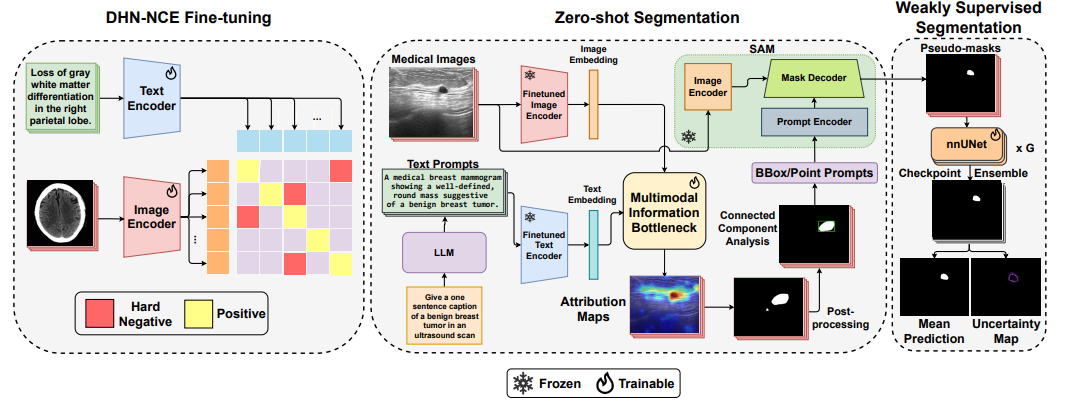
\includegraphics[width=\linewidth,keepaspectratio]{SoDoKhoiChiTiet.png}
\captionof{figure}{\normalfont Sơ đồ kiến trúc luồng dữ liệu từ embedding đa phương thức, saliency map M2IB và sinh segmentation mask bằng SAM~\cite{ref1}.}
\label{fig:dataflow}
\end{center}
\vspace{0.3em}

\subsection{Các thành phần chính trong Pipeline}

\begin{enumerate}
    \item Medical Image (Ảnh y tế đầu vào): Ảnh 2D từ các phương thức chụp chiếu, được biểu diễn dưới dạng ma trận điểm ảnh $I$.
    \item Text Prompt (Gợi ý văn bản): Chuỗi ký tự tự nhiên mô tả mục tiêu cần phân đoạn (ví dụ: ``breast tumor'', ``lung nodule''). Văn bản này được xử lý thông qua bộ mã hóa của BioMedCLIP~\cite{ref3} để sinh ra text embedding.
    \item BioMedCLIP (Vision-Language Base Model): Khác với CLIP thông thường vốn được huấn luyện trên ảnh tự nhiên, BioMedCLIP~\cite{ref3} được tiền huấn luyện trên khoảng 15 triệu cặp ảnh-văn bản y sinh từ cơ sở dữ liệu PubMed. Nhờ đó, mô hình sở hữu khả năng liên kết ngữ nghĩa y khoa, chuyển đổi ảnh $I$ thành visual embedding và câu lệnh văn bản thành text embedding tương ứng trong cùng một không gian ẩn (shared latent space).
    \item M2IB (Multi-modal Information Bottleneck): Đây là thành phần cốt lõi tạo nên tính đột phá. M2IB~\cite{ref7} tối đa hóa lượng thông tin tương hỗ (Mutual Information) giữa visual embedding và text embedding, đồng thời loại bỏ các thành phần nhiễu không liên quan trong ảnh gốc. Kết quả của M2IB là một bản đồ nhiệt biểu diễn sự chú ý (Attention/Saliency Map), chỉ rõ tọa độ không gian ẩn chứa thực thể được mô tả trong văn bản gợi ý.
    \item SAM (Segment Anything Model): Mô hình nền tảng phân đoạn ảnh của Meta. SAM~\cite{ref2,ref4} nhận đầu vào là ảnh gốc cùng các điểm gợi ý hoặc hộp bao được sinh tự động thông qua cơ chế phân ngưỡng bản đồ chú ý từ khối M2IB~\cite{ref7}.
    \item Segmentation Mask (Mask phân đoạn): SAM~\cite{ref2,ref4} thực hiện giải mã (decode) các cấu trúc hình học và biên giới pixel để trả về kết quả phân đoạn nhị phân cuối cùng, phân tách rạch ròi vùng tổn thương và mô lành.
\end{enumerate}

\subsection{Hàm mất mát cải tiến DHN-NCE}

Một đóng góp lý thuyết của phiên bản v2 là việc áp dụng hàm mất mát Decoupled Hard Negative Noise Contrastive Estimation (DHN-NCE)~\cite{ref1} ở giai đoạn tinh chỉnh BioMedCLIP~\cite{ref3}. Hàm DHN-NCE~\cite{ref1} giải quyết hiệu quả hiện tượng liên kết âm (negative-coupling effect) bằng cách loại bỏ mẫu dương khỏi mẫu số của biểu thức tương phản, giúp tối ưu hóa bộ nhớ và tăng cường khả năng phân biệt giữa các tổn thương y khoa có hình thái tương đồng nhưng bản chất bệnh lý khác nhau.

%==============================================================================
% references.tex — Tài liệu tham khảo (được \input từ main.tex)
\begin{thebibliography}{8}

\bibitem{ref1}
T. Koleilat, H. Asgariandehkordi, H. Rivaz, and Y. Xiao,
``MedCLIP-SAMv2: Towards Universal Text-Driven Medical Image Segmentation,''
\textit{arXiv preprint arXiv:2409.19483}, 2024.
Available: \url{https://arxiv.org/abs/2409.19483}

\bibitem{ref2}
Meta AI,
``Segment Anything Model (SAM),''
GitHub Repository, 2023.
Available: \url{https://github.com/facebookresearch/segment-anything}

\bibitem{ref3}
S. Zhang, Y. Xu, N. Usuyama, \textit{et al.},
``Large-Scale Bi-Modal Pre-training for Public Medical Imaging and Text (BioMedCLIP),''
Microsoft Research, 2023.
Available: \url{https://arxiv.org/abs/2303.00915}

\bibitem{ref4}
A. Kirillov, E. Mintun, N. Ravi, \textit{et al.},
``Segment Anything,''
\textit{Proceedings of the IEEE/CVF International Conference on Computer Vision (ICCV)}, 2023.

\bibitem{ref5}
F. Milletari, N. Navab, and S. Ahmadi,
``V-Net: Fully Convolutional Neural Networks for Volumetric Medical Image Segmentation,''
\textit{2016 Fourth International Conference on 3D Vision (3DV)}, 2016.

\bibitem{ref6}
O. Ronneberger, P. Fischer, and T. Brox,
``U-Net: Convolutional Networks for Biomedical Image Segmentation,''
\textit{Medical Image Computing and Computer-Assisted Intervention (MICCAI)}, 2015.

\bibitem{ref7}
M. Wang, T. Rudner, and A. G. Wilson,
``Visual Explanations of Image-Text Representations via Multi-Modal Information Bottleneck Attribution,''
\textit{Advances in Neural Information Processing Systems (NeurIPS)}, 2023.

\bibitem{ref8}
X. Li, H. Gu, M. Zhang, \textit{et al.},
``PPBoost: Progressive Prompt Boosting for Text-Driven Medical Image Segmentation,''
\textit{arXiv preprint arXiv:2511.21984}, 2025.
Available: \url{https://arxiv.org/abs/2511.21984}

\end{thebibliography}


\end{document}
